\chapter{Windowsの基本操作}

\section{ウェブブラウザ}
\subsection{ウェブブラウザとインターネット}
Windowsには Internet Explorerというブラウザがデフォルトでインストールされている。
また、京都大学のPC端末にはMozilla Firefox というブラウザもインストールされている。
両者の基本機能は同じであるが、使い勝手が少し異なる。好みのものを利用すること。

ブラウザの上の方には、閲覧しているウェブサイトのURL (Uniform Resource Locator, 通称、アドレス)が記載してある。
URL の最後は意味があり、最後の2文字は
\begin{itemize}
\item \url{jp} = 日本、
\item \url{uk} = イギリス、
\item \url{fr} = フランス、
\item \url{de} = ドイツ、
\end{itemize}
など、国の名前に対応しており、その前の2文字は
\begin{itemize}
\item \url{co} = 企業、
\item \url{ac} = 大学・研究機関、
\item \url{go} = 政府機関、
\item \url{ne} = 通信関係、
\item \url{or} = その他の機関
\end{itemize}
など、組織の種別に対応している。
ただし、アメリカだけは特別で、国名に当たる部分は省略した上で、最後を3文字で表記することになっている。この3文字はそれぞれ
\begin{itemize}
\item \url{com} = 企業
\item \url{edu} = 大学・研究機関
\item \url{gov} = 政府機関
\item \url{net} = 通信関係
\item \url{org} = その他の機関
\end{itemize}
などのように対応している。

\subsubsection{課題}
\begin{enumerate}
\item ブラウザ(Internet Explorer)を起動する。(デスクトップにあるアイコンをダブルクリック)
\item 京都大学内のホームページ(HP)を知る。

   →京都大学のHP (http://www.kyoto-u.ac.jp/ja) を開く。

   →お気に入りに追加する。
\item 上の「教育・学生支援」にカーソルを合わせるとでてくる「その他学生生活支援」をクリックする。
\item 生活面の諸注意の中の「諸注意」をクリックし、サイト内の情報を熟読すること。
\end{enumerate}

\subsection{違法コピー・ダウンロードの禁止(重要!!)}
サイト上の絵や写真、音楽、映像などを著作権者の許可なく無断でコピー、ダウンロードすることは著作権法に違反し、10年以下の懲役または1,000万円以下の罰金が科せられる。
これまでは、私的利用に限りコピーやダウンロードが認められてきたが、平成22年1月1日に改正著作権法が施行され、たとえ私的であっても違法にアップロードされたものをダウンロードできなくなった。
例えば、YouTube などでテレビドラマなどを見ることも違法となるので、注意すること!!
特に、京都府警のサイバーポリスは優秀で、過去に何人も摘発されている。

違法コピー・ダウンロードはしない!

\subsection{e-learning による情報倫理の学習}
Web は非常に便利なものであるが、ルールを守って使用する義務がある。
つまり、「情報倫理」をきちんと学ぶ必要がある。
京都大学では、e-learning による情報倫理学習コンテンツを国立情報学研究所(NII)が提供する『学認連携 Moodle 講習サイト』により提供している。
デスクトップのショートカット、又は下記の URL から 教育用計算機システムの ID およびパスワードを入力し、ログインする。「学生のための情報環境活用マニュアル」も参照。
\url{http://www.iimc.kyoto-u.ac.jp/ja/services/ismo/e-Learning/}

\subsubsection{課題6}
京都大学情報システム利用規則とセキュリティのテキスト教材で学習したのち、修了テストを行い、その修了画面をPrtScr を使ってコピーしなさい。
次に、スタート→すべてのプログラム→アクセサリ→ペイントでペイントを立ち上げる。
そこに、コピーした画像をペーストし、rinri2015-00000000.jpg というファイル名を付けて M ドライブに保存しなさい。(00000000 の部分には学籍番号を入れること。)

補足:PrtScr は画面全体をコピーすることができる。アクティブな画面のみをコピーしたい場合は、Alt + PrtScr を使うとよい。

\begin{figure}
\centering
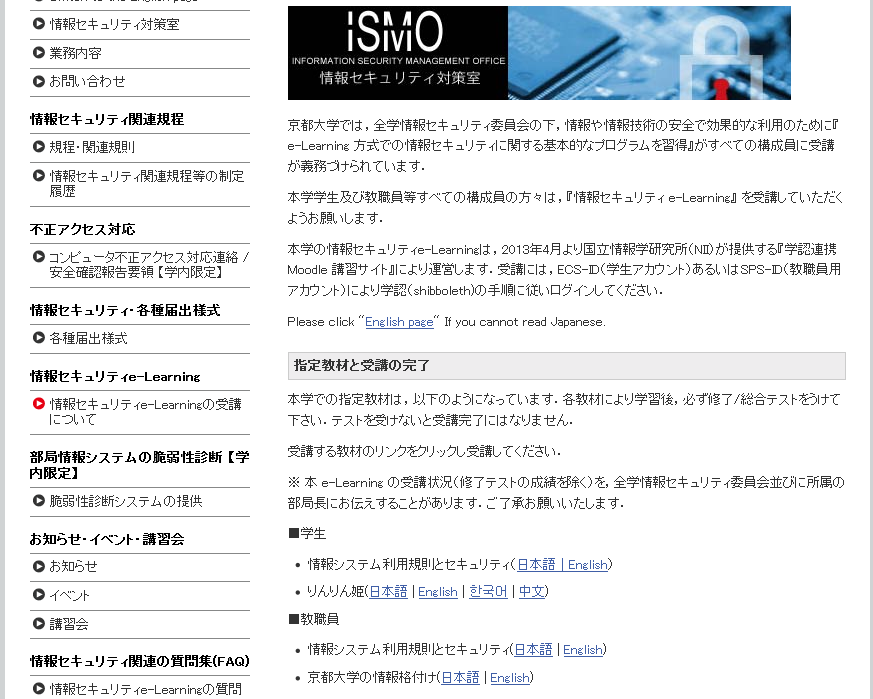
\includegraphics[width=13cm]{TeX_files/figs2/e-learning.png}
\caption{
\label{fig:e-learning}
e-learningへのリンク。右側下部の 学生 > 情報システム利用規則とセキュリティ をクリックする。
}

\end{figure}
\section{電子メール(ウェブメール)}
\subsection{はじめに}
最近は、Lineなどインスタント・メッセンジャーが広く利用されているが、
大学や会社などでは電子メールは一つの公式な文書である。
そのため、ここでは京都大学が提供する電子メールサービスである KUMOI の使い方を学ぶとともに、電子メールを送る際のマナーについても学ぶ。

\subsection{KUMOI}
京都大学情報環境機構ではMicrosoft社が運営するOffice365(Microsoft Office 365 for education)を活用した電子メールサービスを提供している。
これは京都大学に在籍する人は、申請すれば誰でも使用できるので利用するとよい(みなさんはすでに申請済みのはずである)。
ウェブメールは学外(家など)からもメールの受信・送信ができるので便利である。
Internet Explorer もしくは Mozilla Firefox をダブルクリックし、下記のURLを入力し、KUMOI のログイン画面を開く。 

\url{https://mail.st.kyoto-u.ac.jp/LiveLogin/}

ECS-ID、パスワードを入力し、ログインする(詳細は「学生のための情報環境活用マニュアル」8.学生用電子メールサービスの利用方法を参照。)

\begin{figure}
\centering
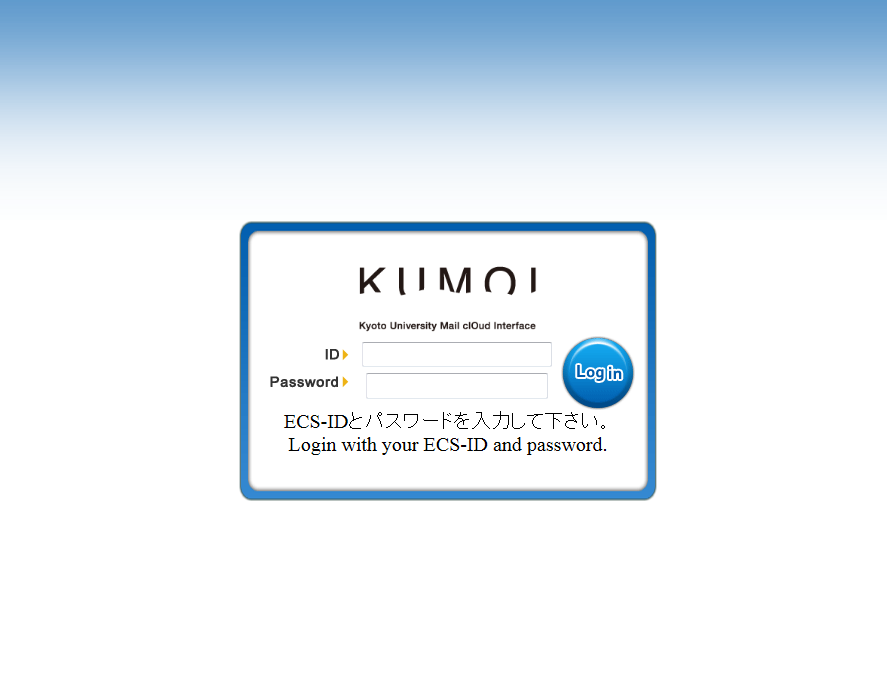
\includegraphics[width=13cm]{TeX_files/figs2/Kumoi.png}
\caption{
\label{fig:Kumoi}
e-learningへのリンク。右側下部の 学生 > 情報システム利用規則とセキュリティ をクリックする。
}
\end{figure}

\subsection{署名}
 電子メールには「署名」という機能がある。署名には名前や連絡先を記載し、一度作成して設定しておけば、送信するメールに自動的に添付されるので便利である。

\begin{enumerate}
\item KUMOIの(オプション)→(すべてのオプションを表示)→(設定)→(メール)と移動し、(電子メールの署名)ボックスに署名を入力する。。

<署名の例>

**********************

 京都大学工学部 物理工学科 1回生 T09

 藤井 恵介 (ふじい けいすけ)

 学籍番号:0000000000

E-mail::xxxxxxxx@st.kyoto-u.ac.jp

**********************

\item 送信メッセージに自動的に署名を追加する)チェックボックスをオンにする(これを忘れると、署名が添付されない。)
\end{enumerate}

\subsection{電子メールにおけるマナー}
電子メールは一種の手紙であるので、Lineのメッセージように宛名等を省いて、用件だけ書くようなことはしない。
電子メールのマナーについては、特に下記の事に気を付けること。
\begin{itemize}
\item 差出人を明らかにする。
\item 件名を必ず書く。
\item 本文の始めに誰に宛てたメールかを必ず書く。
\item 段落が変わるような場所には1行空行をはさむ。
\item 丁寧な言葉づかいを心がける。特に、目上の人には気を付ける。

<例>

○○先生

(1行あける)

物理工学科1回生の××です。

情報基礎演習の課題をお送りします。

よろしくお願いいたします。

\item あまり大きなサイズの添付ファイルを送らない。(京都大学のサーバは10MB程度なら送ることができるが、相手が受け取れない可能性がある。)
\item 相手が表示できる形式のファイルで送信する。(pdf ファイルであれば問題ない。)
\item パスワード、クレジットカード番号などの機密情報は電子メールに記載しない。

\end{itemize}

\subsubsection{【課題1】}
上の手順に従って、自分の署名を作成せよ。署名には名前、ふりがな、学籍番号、クラス、メールアドレスを記載すること。作成が終わったら、送信メールに署名を追加するのを忘れないようにすること。次に、メールを作成し、隣の人にメールを送ってみよ。件名、宛名等を必ず書くこと。本文に作成した署名が入っていることを確認すること。メールを受け取ったら、隣の人に返信してみよ。(返事を書いて送る。)

\subsubsection{【課題2】}
間違ったアドレスに(例えば、自分のアドレスの最後のjpを消して)メールを送ってみよ。しばらくすると、MAILER-DAEMON@MAILER-DAEMON という差出人からエラーメッセージが届くことを確認せよ。
このメールが送られてきた場合は、相手にメールが届いていないので、アドレス等を確認してメールを送り直す必要がある。


\subsubsection{【課題3】}
Web上での情報検索を駆使して、以下の問に答えよ。
解答の作成にはメモ帳を利用し、ファイル名は kadai110407-00000000.txt とすること。110407 の部分には今日の日付を、00000000 の部分は自分の学籍番号を入れること。

問1)現在の京都大学総長のフルネームは?

問2)京都大学の創設は何年?

問3)平成28年度前期の試験期間はいつからいつまでか?

問4)京都大学にある学部を全て答えよ。

問5)現在のアメリカ大統領、バラク・オバマの実父はどこの国の出身?

問6)USBメモリのUSBとは何の略?

問7)「ナノ」とは10の何乗のこと?

問8)プランク定数の値は?(単位とともに答えよ。)

問9)銀閣寺および金閣寺の正式名はそれぞれ何か?

問10)マイクロソフトの本社は何州何市にあるか?
